\documentclass[tikz,border=4pt]{standalone}

\usepackage[T1]{fontenc}
\renewcommand{\rmdefault}{ptm}
\usetikzlibrary{arrows.meta,positioning}

\definecolor{Ink}{HTML}{1F2937}
\definecolor{DataFill}{HTML}{EDF1F4}
\definecolor{DataEdge}{HTML}{4F5D6B}
\definecolor{ProcessFill}{HTML}{E8F1F7}
\definecolor{ProcessEdge}{HTML}{2A6F9E}
\definecolor{ModelFill}{HTML}{F8EBDD}
\definecolor{ModelEdge}{HTML}{B85C1E}
\definecolor{OpticsFill}{HTML}{EAF2EC}
\definecolor{OpticsEdge}{HTML}{4F7A5A}

\tikzset{
  flow/.style={-{Latex[length=1.8mm,width=1.25mm]}, draw=Ink, line width=0.8pt},
  datagroup/.style={draw=DataEdge, fill=white, rounded corners=1.4pt, line width=0.8pt},
  group/.style={draw=ProcessEdge, fill=white, rounded corners=1.4pt, line width=0.8pt},
  modelgroup/.style={draw=ModelEdge, fill=white, rounded corners=1.4pt, line width=0.8pt},
  opticsgroup/.style={draw=OpticsEdge, fill=white, rounded corners=1.4pt, line width=0.8pt},
  data/.style={draw=DataEdge, fill=DataFill, rounded corners=1.2pt, line width=0.8pt,
    align=center, font=\rmfamily\fontsize{7.2}{8.3}\selectfont, inner sep=2.2pt},
  process/.style={draw=ProcessEdge, fill=ProcessFill, rounded corners=1.2pt, line width=0.75pt,
    align=center, font=\rmfamily\fontsize{7.0}{8.0}\selectfont, inner sep=1.8pt},
  learned/.style={draw=ModelEdge, fill=ModelFill, rounded corners=1.2pt, line width=0.75pt,
    align=center, font=\rmfamily\fontsize{7.0}{8.0}\selectfont, inner sep=1.8pt},
  optics/.style={draw=OpticsEdge, fill=OpticsFill, rounded corners=1.2pt, line width=0.8pt,
    align=center, font=\rmfamily\fontsize{7.0}{8.0}\selectfont, inner sep=2.0pt},
  grouptitle/.style={font=\rmfamily\bfseries\fontsize{7.2}{8.2}\selectfont, align=center},
}

\begin{document}
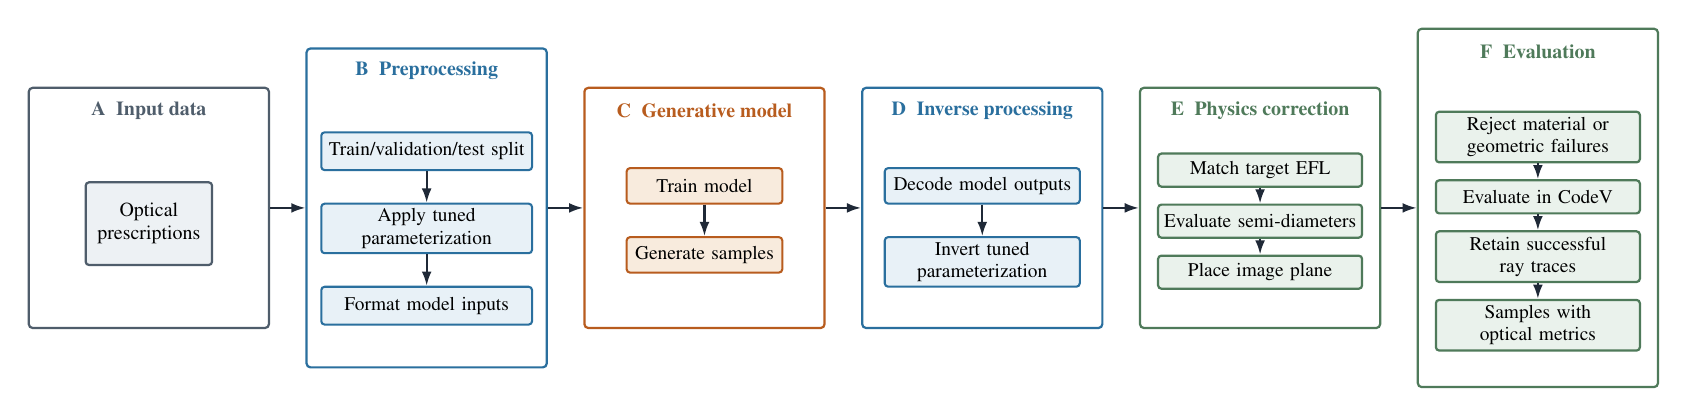
\begin{tikzpicture}[node distance=4.5mm]
  % Every stage uses the same heading-within-container structure.
  \node[datagroup, minimum width=3.05cm, minimum height=3.05cm] (dataStage) {};
  \node[group, minimum width=3.05cm, minimum height=4.05cm, right=of dataStage] (pre) {};
  \node[modelgroup, minimum width=3.05cm, minimum height=3.05cm, right=of pre] (model) {};
  \node[group, minimum width=3.05cm, minimum height=3.05cm, right=of model] (inverse) {};
  \node[opticsgroup, minimum width=3.05cm, minimum height=3.05cm, right=of inverse] (physics) {};
  \node[opticsgroup, minimum width=3.05cm, minimum height=4.55cm, right=of physics] (codev) {};

  \node[grouptitle, text=DataEdge] at ([yshift=-3.0mm]dataStage.north) {A\; Input data};
  \node[grouptitle, text=ProcessEdge] at ([yshift=-3.0mm]pre.north) {B\; Preprocessing};
  \node[grouptitle, text=ModelEdge] at ([yshift=-3.0mm]model.north) {C\; Generative model};
  \node[grouptitle, text=ProcessEdge] at ([yshift=-3.0mm]inverse.north) {D\; Inverse processing};
  \node[grouptitle, text=OpticsEdge] at ([yshift=-3.0mm]physics.north) {E\; Physics correction};
  \node[grouptitle, text=OpticsEdge] at ([yshift=-3.0mm]codev.north) {F\; Evaluation};

  % Data and operations are positioned beneath their stage headings.
  \node[data, text width=1.45cm, minimum height=1.05cm] (canonical) at ([yshift=-2.0mm]dataStage.center)
    {Optical\\prescriptions};
  \node[process, text width=2.55cm, minimum height=0.48cm] (split) at ([yshift=7.2mm]pre.center)
    {Train/validation/test split};
  \node[process, text width=2.55cm, minimum height=0.48cm, below=4.0mm of split] (repr)
    {Apply tuned\\parameterization};
  \node[process, text width=2.55cm, minimum height=0.48cm, below=4.0mm of repr] (format)
    {Format model inputs};

  \node[learned, text width=1.85cm, minimum height=0.45cm] (train) at ([yshift=2.8mm]model.center) {Train model};
  \node[learned, text width=1.85cm, minimum height=0.45cm, below=4.0mm of train] (sample) {Generate samples};

  \node[process, text width=2.35cm, minimum height=0.45cm] (modelinv) at ([yshift=2.8mm]inverse.center)
    {Decode model outputs};
  \node[process, text width=2.35cm, minimum height=0.45cm, below=4.0mm of modelinv] (opticsinv)
    {Invert tuned\\parameterization};

  \node[optics, text width=2.45cm, minimum height=0.42cm] (eflOp) at ([yshift=4.8mm]physics.center)
    {Match target EFL};
  \node[optics, text width=2.45cm, minimum height=0.42cm, below=2.0mm of eflOp] (apertureOp)
    {Evaluate semi-diameters};
  \node[optics, text width=2.45cm, minimum height=0.42cm, below=2.0mm of apertureOp] (imageOp)
    {Place image plane};

  \node[optics, text width=2.45cm, minimum height=0.42cm] (inputFilterOp) at ([yshift=9.0mm]codev.center)
    {Reject material or\\geometric failures};
  \node[optics, text width=2.45cm, minimum height=0.42cm, below=2.0mm of inputFilterOp] (codevOp)
    {Evaluate in CodeV};
  \node[optics, text width=2.45cm, minimum height=0.42cm, below=2.0mm of codevOp] (rayFilterOp)
    {Retain successful\\ray traces};
  \node[optics, text width=2.45cm, minimum height=0.42cm, below=2.0mm of rayFilterOp] (metricsOp)
    {Samples with\\optical metrics};

  % Uniform internal and stage-to-stage flow.
  \draw[flow] (split.south) -- (repr.north);
  \draw[flow] (repr.south) -- (format.north);
  \draw[flow] (train.south) -- (sample.north);
  \draw[flow] (modelinv.south) -- (opticsinv.north);
  \draw[flow] (eflOp.south) -- (apertureOp.north);
  \draw[flow] (apertureOp.south) -- (imageOp.north);
  \draw[flow] (inputFilterOp.south) -- (codevOp.north);
  \draw[flow] (codevOp.south) -- (rayFilterOp.north);
  \draw[flow] (rayFilterOp.south) -- (metricsOp.north);
  \draw[flow] (dataStage.east) -- (pre.west);
  \draw[flow] (pre.east) -- (model.west);
  \draw[flow] (model.east) -- (inverse.west);
  \draw[flow] (inverse.east) -- (physics.west);
  \draw[flow] (physics.east) -- (codev.west);

\end{tikzpicture}
\end{document}
